\section{What's wrong with Paxos?}
\label{motivation:paxos}

\begin{figure*}
\centering
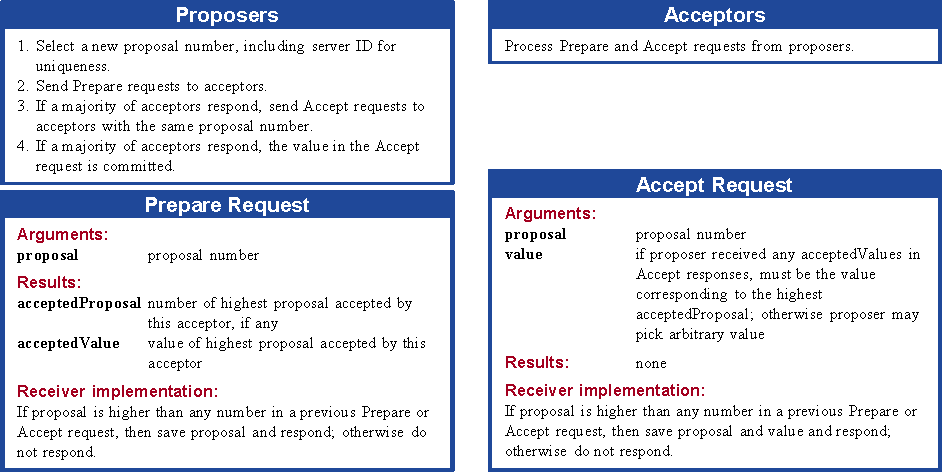
\includegraphics[scale=0.95]{motivation/paxossummary}
\vcaption[summary of the single-decree Paxos protocol]{
Summary of the single-decree Paxos consensus protocol.
See \cite{Lamport:2001} for a detailed explanation.
}
\label{fig:motivation:paxos:basic}
\end{figure*}


Over the last ten years, Leslie Lamport's Paxos protocol~\cite{Lamport:1998}
has become almost synonymous with consensus: it is the protocol
most commonly taught in courses, and most implementations of consensus
use it as a starting point. Paxos first defines a protocol capable
of reaching agreement on a single decision, such as a single replicated
log entry.  We refer to this subset as \emph{single-decree Paxos}.
Paxos then combines multiple instances of this protocol to facilitate
a series of decisions such as a log (\emph{Multi-Paxos}).
Single-decree Paxos is summarized in
Figure~\ref{fig:motivation:paxos:basic}, and Multi-Paxos is summarized
in Figure~\ref{fig:appendix:userstudy:paxossummary4}.
Paxos ensures safety and liveness (it eventually reaches consensus,
assuming an adequate failure detector
is used to avoid proposer livelock), and its correctness has been proven.
Multi-Paxos is efficient in the normal case, and Paxos supports changes
in cluster membership~\cite{Lorch:2006}.

Unfortunately, Paxos has two significant drawbacks.  The first drawback is
that Paxos is exceptionally difficult to understand. The full
explanation~\cite{Lamport:1998} is notoriously opaque; few
people succeed in understanding it, and only with great effort.
As a result, there have been several attempts to explain Paxos
in simpler terms~\cite{Lamport:2001, Lampson:1996, Lampson:2001}.
These explanations focus on the single-decree subset,
yet they are still challenging.
In an informal survey of attendees at NSDI 2012, we found few people who
were comfortable with Paxos, even among seasoned researchers.
We struggled with Paxos ourselves; we were not able to understand
the complete protocol
until after reading several explanations
and designing our own alternative protocol, a process that took
almost a year.

We hypothesize that Paxos' opaqueness stems from its choice of the
single-decree subset as its foundation. Single-decree
Paxos is dense and subtle: it is divided into two stages that do
not have simple intuitive explanations and cannot be understood
independently. Because of this, it is difficult to
develop intuitions about why the single-decree protocol works.
The composition rules for Multi-Paxos add significant additional
complexity and subtlety. We believe that the overall
problem of reaching consensus on multiple decisions (i.e., a log instead
of a single entry) can be decomposed in other ways that are more
direct and obvious.

The second problem with Paxos is that it does not provide a good
foundation
for building practical implementations. One reason is that
there is no widely agreed-upon algorithm for Multi-Paxos.
Lamport's descriptions are mostly about single-decree Paxos;
he sketched possible approaches to Multi-Paxos, but many
details are missing. There have been several attempts to flesh out and
optimize Paxos, such as \cite{Mazieres:2007}, \cite{Renesse:2011},
and \cite{Kirsch:2008},
but these differ from each other and from Lamport's sketches.
Systems such as Chubby~\cite{Chandra:2007} have implemented
Paxos-like algorithms, but in most cases their details have not been
published.


Furthermore, the Paxos
architecture is a poor one
for building practical systems; this
is another consequence of the
single-decree decomposition. For example, there is
little benefit to
choosing a collection of log entries independently and then melding
them into a sequential log; this just adds complexity.  It is simpler
and more efficient to design a system around a log, where new
entries are appended sequentially in a constrained order.
Another problem is that Paxos
uses a symmetric peer-to-peer approach at its core (though it
also suggests a weak form of leadership as a performance
optimization). This makes
sense in a simplified world where only one decision will be made,
but few practical systems use this approach. If a series of decisions
must be made, it is simpler and faster to first elect a
leader, then have the leader coordinate the decisions.
(Chapter~\ref{related} discusses Egalitarian Paxos, a recent
variant of Paxos that does not use a leader but in some situations can
be more efficient than algorithms that do; however, this algorithm is
much more complex than leader-based algorithms.)

As a result, practical systems bear little resemblance to Paxos.
Each implementation begins with Paxos, discovers the difficulties in
implementing it, and then develops a significantly different architecture.
This is time-consuming and error-prone, and the difficulties of
understanding Paxos exacerbate the problem.
Paxos' formulation may be a good one for proving theorems about
its correctness, but real implementations are so
different from Paxos that the proofs have little value. The following
comment from the Chubby implementers is typical:

{\defaultleftmargin{4em}{}{}{}
\begin{quote}
There are significant gaps between the description of the Paxos
algorithm and the needs of a real-world system\dots. the final system
will be based on an unproven protocol~\cite{Chandra:2007}.
\end{quote}
}

Because of these problems, we concluded that Paxos does not provide
a good foundation either for system building or for education.
Given the importance of consensus in large-scale software
systems, we decided to see if we could design an alternative consensus
algorithm with better properties than Paxos.  \name{} is the result
of that experiment.


%

